\subsection{Software Design}
This section covers the bulk of our software design in the report as we mainly create artifacts in this sprint to help us during coding. First, we'll show how we use UML artifacts to gain insight into complicated methods and tasks our system should support. Then we'll describe and discuss how we use the GRASP principles \cite[p.~271, p.~413]{OOAD}. And finally, we'll highlight the use of some design patterns not included in GRASP but relevant to our non-functional requirements.
\subsubsection{Static Object Modelling}
As described earlier, we try to model our system in a Client-Server pattern. While a user can store all his files offline, the remote storage should avoid redundancy and thus only store each file once no matter how many users are sharing it. This means that a client's representation of a file should differ from the server. Additionally, even though the system is meant to be a proof of concept, we want to design modules for extensibility. This means that including support for other files than documents (for example binary files) should be easy to implement in a future release. We design with this in mind when doing our database design and thus our corresponding ‘mapped objects'. Below is a ‘class diagram' modeling our database entities:\\
\begin{figure}[h]
  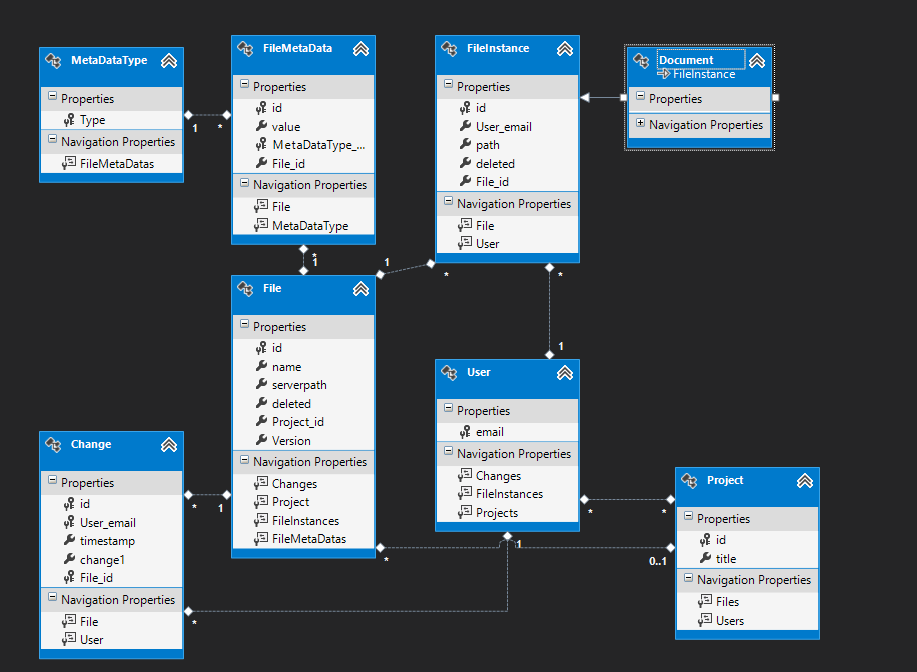
\includegraphics[width=\textwidth,natwidth=793,natheight=635]{illustrations/entitymodel.png}
  \caption{Entity Model}
  \label{entitymodel2}
\end{figure}
Although the model is more resembling to a relational model than an actual UML class diagram, we still find it useful in regards to describing our way of persisting data. Each File has a list of changes, which record a user, a time and a description of the change. Each File list to a number of FileInstances, which contains user-specific file information. A Document entity, which we use in the program to edit and show text, inherits directly from FileInstance. Additionally, each File contains a number of FileMetaData, which can be specific for the type of file.\\
The model does not describe any properties of the classes, as they almost only contain data. Only methods that represents the data as a text string is contained.
\subsubsection{Static Persistence View}
When designing the persistence part of the model, we initially build a list of interfaces so other parts of the system such as a controller or a network module can develop and compile their code against the persistence module. These interfaces are modeled in Visual Studio so we can also generate method signatures and classes from the definitions. A part of the interface diagram is shown below:\\
\begin{figure}[H]
  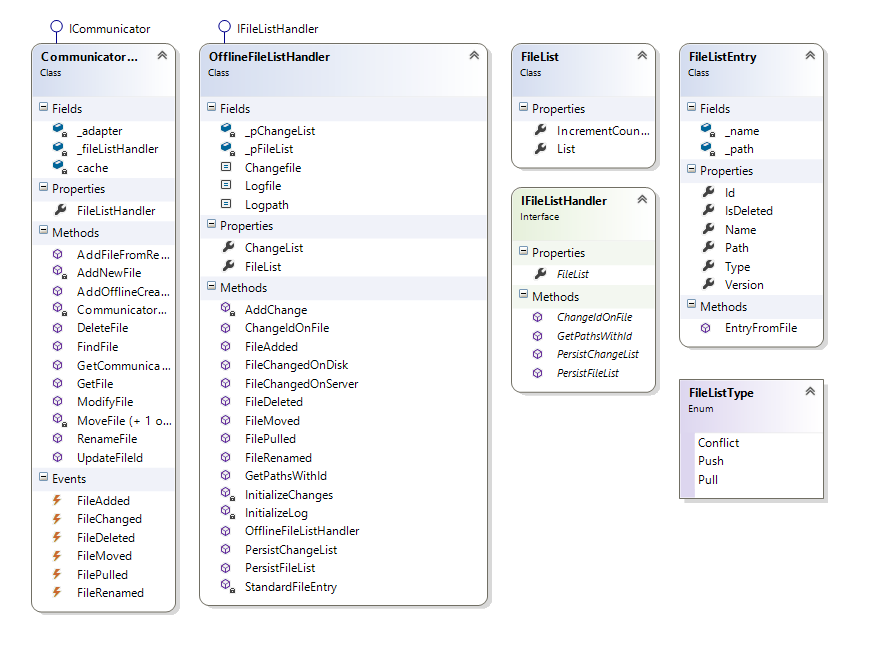
\includegraphics[width=\textwidth]{illustrations/persistenceclasses.png}
  \caption{Persistence Classes}
  \label{persistenceclasses}
\end{figure}
The models in Visual Studio resembles UML notation but with a few differences. For example, the private modifier is shown with a little lock instead of a ‘-'. However, the benefits of having a virtual model (such as code lookup and method documentation on hover) greatly outweighs the change in notation, and we have chosen this advantage over showing the proper UML.\\
A full class diagram will be presented and discussed in Sprint 3 as code documentation.
\subsubsection{Dynamic Modelling}
Following our design of the data-containing classes, we move on to modelling the complex runtime behaviour of our system. We make communication diagrams of the program-flow in the four use cases initially made in the first sprint. The purpose of these diagrams is mainly:
\begin{itemize}
\item Reveal classes needed to facilitate complex runtime behavior. 
\item Highlight places in the system where applying design patterns might be useful.
\item Give members of the Scrum team a common foundation for working on different parts of the system at the same time (interfaces)
\end{itemize}
We will present how we make interaction diagrams as a case study of one our use cases.
\subsubsection{Case: Synchronization}
Below is an example of an UML communication diagram made to support a process as described in a use case, U\#2. Please note that the diagram illustrates the design as we thought it out at the start of the sprint. A section regarding the diagrams used for ‘real' code documentation is presented in Sprint 3. \\
The diagram illustrates the need for several interacting modules, each with a well-defined API, each module briefly described:\\
\begin{itemize}
\item An administrator module, serving as an entry point to the model, receiving and redirecting requests from the user interface
\item A persistence module, which is responsible for saving and retrieve files from storage, possibly reuseable on both the client and the server (if they use a similar file system)
\item A marshalling module, which is a technical service for converting objects to a persistent data format. This module should be developed
independently of the persistent storage so it is potentially reuseable. 
\item A networking module, which is responsible for sending and receiving files and logs through a network protocol.
\end{itemize}
[Appendix, Illustrations, \ref{CD5A} and \ref{CD5B}, page \pageref{CD5A} and \pageref{CD5B}]\\
\newline
\newline
Client objects should not be dependent on more than one interface on the server side. This shows in the sequence diagram by the many method arrows that are interrupted by object lifelines. As the server logic contains concurrent programming to allow for separate client requests at the same time, we expand the concrete logic in a UML activity diagram. This diagram is shown in [Appendix, Illustrations, \ref{activitydiagram}, page \pageref{activitydiagram}]\\
\newline
The diagram notates threads as different swimlanes. Each request from a client is treated separately and concurrently. Additionally, each synchronization process relates to a specified user. This means that several clients can access the server at the same time and request synchronization.\\
\subsubsection{Using GRASP principles}
To illustrate how the GRASP principles has helped us create clean, manageable code. We will highlight some areas of the system where we have applied the principles. We'll also briefly discuss the pros and cons of the applied principles. \\
A notable example of how we apply a GRASP principle is the class ClientController.cs (part of the OfflineGUI assembly), which is a controller object. The controller is modeled as a facade controller as opposed to a use case controller \cite[p.~237]{OOAD}.\\
The controller receives input from the user as events and calls the correct methods on the model of the system. A complete separation of the technical services of the model and the GUI is achieved with this construct. However, this also introduces some extra code.\\
\newline
Another example of a GRASP principle in practice is that of the Pure Fabrication \cite[p.~330]{OOAD}. The pattern is applied many times but we highlight the class OfflineFileListHandler.cs. This class does not represent any entity in the domain model, but models a function which we need to synchronize files. The class responsibilities is handling a detailed list of files maintained offline as well as changes made to them. The class is modeled after an interface, IFileListHandler.cs, which allows the module to be potentially reused on the server. The class has a strictly defined  set of responsibilities in that it should only contain and maintain the filelist, but not apply any logic based on the information in the filelist. That responsibility is modeled in other classes such as the OfflineAdministrator.cs\\
\subsubsection{Other design patterns}
The GRASP principles provides a foundation for creating classes that maintain low coupling and high cohesion. In this subsection, we'll discuss how we use other design patterns mainly attributed to the GoF \cite[p.~342]{OOAD}. The patterns are often used several times in the code; we will highlight the examples we think have demonstrational value. In particular, we focus in the model on improving our persistent module by applying patterns.\\
\newline
A keypoint of our software has been extensibility. Following this thought, we want persistent storage to be adaptable and portable. This means each data type is designed to be replaced or handled differently. However, the user interface or any controller should still compile even though significant changes (such as changing persistent storage from a file system to a relational database) were made in the model. We used the Facade pattern to achieve this layer of compile-time safety. The OfflineAdministrator.cs serves as a single entry point for the entire model. The interface that the administrator is simplified as to hide complex functionality. For example, the administrator interface only specifies one method each for getting and retrieving any class or subclass of the FileInstance. However, the lower level interfaces define several methods for doing this as it depends on whether the file was created locally or remotely. 
A drawback of the Facade pattern is that the entry object is crucial to correct program execution. To eliminate potential errors, the class therefore also implements the Singleton pattern. The pattern only allows one object of the class to be instantiated at any time \cite[p.~348]{OOAD}. The benefit of this pattern is that we control access to files on the disk through only one object, avoiding any potential exceptions from simultaneous access attempts. \\
\newline
Another pattern that we like to highlight in the persistence module is the Cache Management \cite[p.~551]{OOAD}. The cache management is done in the class which loads files from disks and when loading, it maintains the file in memory for later use. However, the cache could be improved by for example implementing a caching algorithm. This would be useful if the system should extend its use to other file types like large images.\\
\newline
Part of the Model View Controller pattern which we implement also includes the Observer Pattern \cite[p.~377]{OOAD}. This pattern is easily implemented in C\# by using the delegate and the event constructs. This means that the Windows Forms which we use for user interface publishes user inputs as events without knowing the identity of observers. This causes low coupling. \\
% Michael add stuff here about composite
\newpage